\hypertarget{project-2-report-oled-on-zedboard}{%
\section{Project 2 Report: OLED on
Zedboard}\label{project-2-report-oled-on-zedboard}}

\hypertarget{overview}{%
\subsection{Overview}\label{overview}}

\begin{enumerate}
\def\labelenumi{\arabic{enumi}.}
\tightlist
\item
  Instantiate an AXI-SPI Core in the PL of the Zynq SoC to handle SPI
  communication.
\item
  The PS writes data to the AXI-SPI core via AXI4-Lite.
\item
  The AXI-SPI core in the PL sends the SPI data to the OLED display.
\end{enumerate}

\hypertarget{oled-interfaces}{%
\subsection{OLED Interfaces}\label{oled-interfaces}}

\begin{itemize}
\item
  \textbf{GPIO (Parallel)}: Uses multiple pins to transfer data in
  parallel, offering high-speed communication but requiring many GPIO
  pins, which can be complex to wire and debug.
\item
  \textbf{I2C}: A two-wire serial interface (SDA for data, SCL for
  clock) that is simple to wire and allows multiple devices on the same
  bus but operates at a slower speed compared to SPI, making it ideal
  for simpler displays.
\item
  \textbf{SPI}: Several variations, but generally a two to four wire
  serial interface that provides faster communication than I2C with
  fewer pins than GPIO, striking a balance between speed and pin usage
  for moderately complex displays.
\end{itemize}

This project implements the SPI interface to communicate with the OLED
display.

\hypertarget{arm-advanced-microcontroller-bus-architecture-amba}{%
\subsection{ARM Advanced Microcontroller Bus Architecture
(AMBA)}\label{arm-advanced-microcontroller-bus-architecture-amba}}

The Advanced Microcontroller Bus Architecture (AMBA) is an open-standard
interconnect system developed by ARM for efficient on-chip communication
in System-on-Chip (SoC) designs. Key protocols include:

\begin{enumerate}
\def\labelenumi{\arabic{enumi}.}
\item
  \textbf{AHB (Advanced High-performance Bus)}: High-bandwidth,
  pipelined bus for fast data transfers, ideal for processors and
  high-speed peripherals.
\item
  \textbf{APB (Advanced Peripheral Bus)}: Simplified, low-power bus for
  slower peripherals like GPIOs and timers, with reduced complexity.
\item
  \textbf{AXI (Advanced eXtensible Interface)}: High-performance bus
  supporting multiple masters, separate read/write channels, and
  efficient memory access, used for data-intensive tasks.
\item
  \textbf{ACE (AXI Coherency Extensions)}: Adds cache coherency for
  multi-core systems, crucial for synchronized data access.
\item
  \textbf{CHI (Coherent Hub Interface)}: High-bandwidth protocol for
  data center applications, maintaining data coherency across
  distributed systems.
\end{enumerate}

\hypertarget{axi-advanced-extensible-interface}{%
\subsubsection{AXI (Advanced eXtensible
Interface)}\label{axi-advanced-extensible-interface}}

\begin{enumerate}
\def\labelenumi{\arabic{enumi}.}
\tightlist
\item
  \textbf{AXI3}:

  \begin{itemize}
  \tightlist
  \item
    The original AXI specification.
  \item
    Supports up to 16 data beats per burst.
  \item
    Does not support features like QoS (Quality of Service) and
    user-defined signaling present in later versions.
  \item
    Commonly used in systems where backward compatibility is required.
  \end{itemize}
\item
  \textbf{AXI4}:

  \begin{itemize}
  \tightlist
  \item
    An enhanced version of AXI3, widely used in modern SoCs.
  \item
    Supports up to 256 data beats per burst, increasing data throughput.
  \item
    Adds features like QoS signaling for managing data flow priorities.
  \item
    Supports both high-bandwidth and low-latency requirements, making it
    suitable for high-performance applications.
  \end{itemize}
\item
  \textbf{AXI4-Lite}:

  \begin{itemize}
  \tightlist
  \item
    A simplified, low-resource version of AXI4, supporting only single
    32-bit data transfers.
  \item
    Does not support burst transactions, making it ideal for low-speed,
    low-power peripherals.
  \item
    Commonly used for control registers and simple peripheral
    communications.
  \end{itemize}
\item
  \textbf{AXI4-Stream}:

  \begin{itemize}
  \tightlist
  \item
    Designed for unidirectional, high-throughput data streaming without
    addressing overhead.
  \item
    Does not use address channels, focusing solely on continuous data
    transfer.
  \item
    Ideal for applications requiring high data rates, such as video
    processing, networking, and digital signal processing (DSP).
  \end{itemize}
\item
  \textbf{AXI5}:

  \begin{itemize}
  \tightlist
  \item
    The latest update to AXI, introduced by ARM to improve cache
    coherency and system efficiency.
  \item
    Supports advanced coherency protocols and fault tolerance features
    for high-reliability applications.
  \item
    Mainly used in multi-core systems that require sophisticated memory
    consistency across processors.
  \end{itemize}
\end{enumerate}

\hypertarget{axi4-lite-protocol}{%
\subsection{AXI4-Lite Protocol}\label{axi4-lite-protocol}}

\begin{figure}
\centering
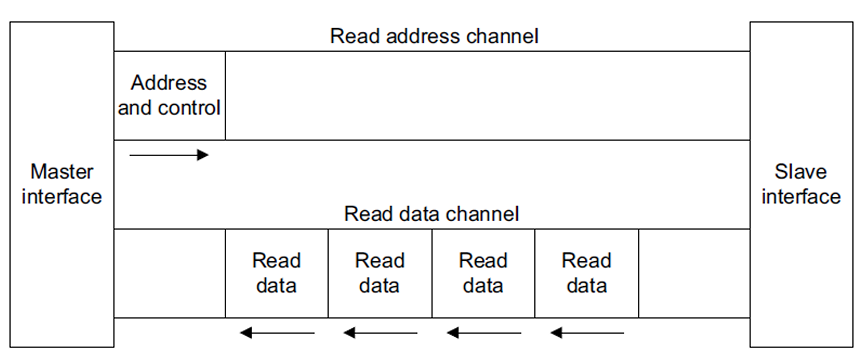
\includegraphics{images/read_channels_diagram.png}
\caption{Read Channels}
\end{figure}

\begin{itemize}
\tightlist
\item
  The \textbf{read address channel} carries addressing information and
  handshaking signals
\item
  The \textbf{read data channel} carries the data values and handshaking
  signals
\end{itemize}

\begin{figure}
\centering
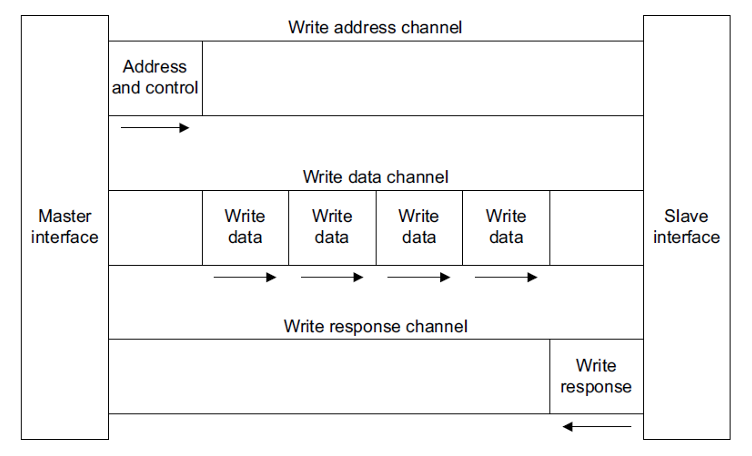
\includegraphics{images/write_channels_diagram.png}
\caption{Write Channels}
\end{figure}

\begin{itemize}
\tightlist
\item
  The \textbf{write address channel} carries addressing information and
  handshaking signals
\item
  The \textbf{write data channel} carries the data values and
  handshaking signals
\item
  The \textbf{write response channel} allows the slave peripheral to
  acknowledge receipt of the data
\end{itemize}

\hypertarget{axi4-lite-ports}{%
\subsubsection{AXI4-Lite Ports}\label{axi4-lite-ports}}

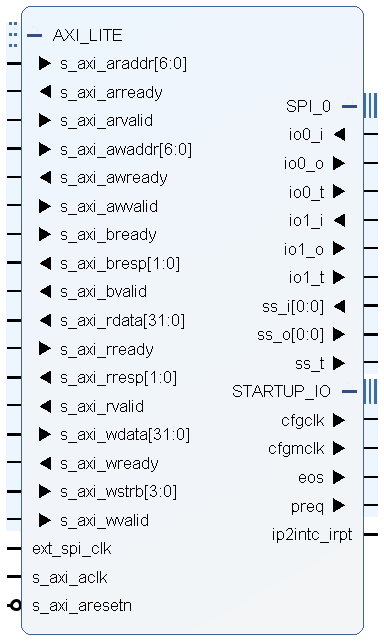
\includegraphics{images/axi_lite_block_diagram.png}\\
\emph{From Vivado AXI Quad SPI IP}

\hypertarget{read-transactions}{%
\subsubsection{Read Transactions}\label{read-transactions}}

\textbf{Handshaking Signals:}

The handshaking signals are based on a simple ``Ready/Valid'' principle:

\begin{itemize}
\tightlist
\item
  ``Ready'' indicates that the recipient is ready to accept data.
\item
  ``Valid'' indicates that the sender has valid data to send.
\end{itemize}

Either state can be asserted first:

\begin{quote}
``A frequently misunderstood use of the Valid and Ready signals, and one
which often results in incorrect and illegal implementations of the
AXI4-lite protocol, is the assumption that the sender can/must wait for
``Ready'' to be asserted by the receiver before it asserts its ``Valid''
signal. This is an illegal use of the handshaking signals and can result
in a deadlock situation arising. Ready can be asserted before Valid, but
the sender must never wait for Ready as a pre-condition to commencing
the transaction.''
\end{quote}

\hypertarget{axi4-lite-read-address-channel}{%
\paragraph{AXI4-lite Read Address
Channel}\label{axi4-lite-read-address-channel}}

\begin{longtable}[]{@{}
  >{\raggedright\arraybackslash}p{(\columnwidth - 6\tabcolsep) * \real{0.1230}}
  >{\raggedright\arraybackslash}p{(\columnwidth - 6\tabcolsep) * \real{0.0738}}
  >{\raggedright\arraybackslash}p{(\columnwidth - 6\tabcolsep) * \real{0.0902}}
  >{\raggedright\arraybackslash}p{(\columnwidth - 6\tabcolsep) * \real{0.7131}}@{}}
\toprule\noalign{}
\begin{minipage}[b]{\linewidth}\raggedright
Signal Name
\end{minipage} & \begin{minipage}[b]{\linewidth}\raggedright
Size
\end{minipage} & \begin{minipage}[b]{\linewidth}\raggedright
Driven by
\end{minipage} & \begin{minipage}[b]{\linewidth}\raggedright
Description
\end{minipage} \\
\midrule\noalign{}
\endhead
\bottomrule\noalign{}
\endlastfoot
S\_AXI\_ARADDR & 32 bits & Master & Address bus from AXI interconnect to
slave peripheral. \\
S\_AXI\_ARVALID & 1 bit & Master & Valid signal, asserting that the
S\_AXI\_AWADDR can be sampled by the slave peripheral. \\
S\_AXI\_ARREADY & 1 bit & Slave & Ready signal, indicating that the
slave is ready to accept the value on S\_AXI\_AWADDR. \\
\end{longtable}

\hypertarget{axi4-lite-read-data-channel}{%
\paragraph{AXI4-lite Read Data
Channel}\label{axi4-lite-read-data-channel}}

\begin{longtable}[]{@{}
  >{\raggedright\arraybackslash}p{(\columnwidth - 6\tabcolsep) * \real{0.0946}}
  >{\raggedright\arraybackslash}p{(\columnwidth - 6\tabcolsep) * \real{0.0608}}
  >{\raggedright\arraybackslash}p{(\columnwidth - 6\tabcolsep) * \real{0.0743}}
  >{\raggedright\arraybackslash}p{(\columnwidth - 6\tabcolsep) * \real{0.7703}}@{}}
\toprule\noalign{}
\begin{minipage}[b]{\linewidth}\raggedright
Signal Name
\end{minipage} & \begin{minipage}[b]{\linewidth}\raggedright
Size
\end{minipage} & \begin{minipage}[b]{\linewidth}\raggedright
Driven by
\end{minipage} & \begin{minipage}[b]{\linewidth}\raggedright
Description
\end{minipage} \\
\midrule\noalign{}
\endhead
\bottomrule\noalign{}
\endlastfoot
S\_AXI\_RDATA & 32 bits & Slave & Data bus from the slave peripheral to
the AXI interconnect. \\
S\_AXI\_RVALID & 1 bit & Slave & Valid signal, asserting that the
S\_AXI\_RDATA can be sampled by the Master. \\
S\_AXI\_RREADY & 1 bit & Master & Ready signal, indicating that the
Master is ready to accept the value on the other signals. \\
S\_AXI\_RRESP & 2 bits & Slave & A ``Response'' status signal showing
whether the transaction completed successfully or whether there was an
error. \\
\end{longtable}

\hypertarget{s_axi_rresp-signals}{%
\subparagraph{S\_AXI\_RRESP Signals}\label{s_axi_rresp-signals}}

\begin{longtable}[]{@{}
  >{\raggedright\arraybackslash}p{(\columnwidth - 4\tabcolsep) * \real{0.0815}}
  >{\raggedright\arraybackslash}p{(\columnwidth - 4\tabcolsep) * \real{0.0472}}
  >{\raggedright\arraybackslash}p{(\columnwidth - 4\tabcolsep) * \real{0.8712}}@{}}
\toprule\noalign{}
\begin{minipage}[b]{\linewidth}\raggedright
RRESP State {[}1:0{]}
\end{minipage} & \begin{minipage}[b]{\linewidth}\raggedright
Condition
\end{minipage} & \begin{minipage}[b]{\linewidth}\raggedright
Description
\end{minipage} \\
\midrule\noalign{}
\endhead
\bottomrule\noalign{}
\endlastfoot
00 & OKAY & ``OKAY'' - The data was received successfully, and there
were no errors. \\
01 & EXOKAY & ``Exclusive Access OK'' - This state is only used in the
full implementation of AXI4, and therefore cannot occur when using
AXI4-Lite. \\
10 & SLVERR & ``Slave Error'' - The slave has received the address phase
of the transaction correctly but needs to signal an error condition to
the master. Often results in a retry. \\
11 & DECERR & ``Decode Error'' - This condition is not normally asserted
by a peripheral but can be asserted by the AXI interconnect logic. It
indicates the address doesn't exist in the AXI interconnect address
space. \\
\end{longtable}

\hypertarget{write-transactions}{%
\subsubsection{Write Transactions}\label{write-transactions}}

Write transactions are almost identical to the Read transactions
discussed above, except that the Write Data Channel has one signal that
is different to the Read Data Channel.

\hypertarget{axi4-lite-write-address-channel}{%
\paragraph{AXI4-lite Write Address
Channel}\label{axi4-lite-write-address-channel}}

\begin{longtable}[]{@{}
  >{\raggedright\arraybackslash}p{(\columnwidth - 6\tabcolsep) * \real{0.1027}}
  >{\raggedright\arraybackslash}p{(\columnwidth - 6\tabcolsep) * \real{0.0616}}
  >{\raggedright\arraybackslash}p{(\columnwidth - 6\tabcolsep) * \real{0.0753}}
  >{\raggedright\arraybackslash}p{(\columnwidth - 6\tabcolsep) * \real{0.7603}}@{}}
\toprule\noalign{}
\begin{minipage}[b]{\linewidth}\raggedright
Signal Name
\end{minipage} & \begin{minipage}[b]{\linewidth}\raggedright
Size
\end{minipage} & \begin{minipage}[b]{\linewidth}\raggedright
Driven by
\end{minipage} & \begin{minipage}[b]{\linewidth}\raggedright
Description
\end{minipage} \\
\midrule\noalign{}
\endhead
\bottomrule\noalign{}
\endlastfoot
S\_AXI\_AWADDR & 32 bits & Master & Address bus from AXI interconnect to
slave peripheral. \\
S\_AXI\_AWVALID & 1 bit & Master & Valid signal, asserting that the
S\_AXI\_AWADDR can be sampled by the slave peripheral. \\
S\_AXI\_AWREADY & 1 bit & Slave & Ready signal, indicating that the
slave is ready to accept the value on S\_AXI\_AWADDR. \\
\end{longtable}

\hypertarget{axi4-lite-write-data-channel}{%
\paragraph{AXI4-lite Write Data
Channel}\label{axi4-lite-write-data-channel}}

\begin{longtable}[]{@{}
  >{\raggedright\arraybackslash}p{(\columnwidth - 6\tabcolsep) * \real{0.1007}}
  >{\raggedright\arraybackslash}p{(\columnwidth - 6\tabcolsep) * \real{0.0647}}
  >{\raggedright\arraybackslash}p{(\columnwidth - 6\tabcolsep) * \real{0.0791}}
  >{\raggedright\arraybackslash}p{(\columnwidth - 6\tabcolsep) * \real{0.7554}}@{}}
\toprule\noalign{}
\begin{minipage}[b]{\linewidth}\raggedright
Signal Name
\end{minipage} & \begin{minipage}[b]{\linewidth}\raggedright
Size
\end{minipage} & \begin{minipage}[b]{\linewidth}\raggedright
Driven by
\end{minipage} & \begin{minipage}[b]{\linewidth}\raggedright
Description
\end{minipage} \\
\midrule\noalign{}
\endhead
\bottomrule\noalign{}
\endlastfoot
S\_AXI\_WDATA & 32 bits & Master & Data bus from the Master / AXI
interconnect to the Slave peripheral. \\
S\_AXI\_WVALID & 1 bit & Master & Valid signal, asserting that the
S\_AXI\_RDATA can be sampled by the Master. \\
S\_AXI\_WREADY & 1 bit & Slave & Ready signal, indicating that the
Master is ready to accept the value on the other signals. \\
S\_AXI\_WSTRB & 4 bits & Master & A ``Strobe'' status signal showing
which bytes of the data bus are valid and should be read by the
Slave. \\
\end{longtable}

\hypertarget{s_axi_wstrb-signals}{%
\subparagraph{S\_AXI\_WSTRB Signals}\label{s_axi_wstrb-signals}}

\begin{longtable}[]{@{}
  >{\raggedright\arraybackslash}p{(\columnwidth - 4\tabcolsep) * \real{0.2043}}
  >{\raggedright\arraybackslash}p{(\columnwidth - 4\tabcolsep) * \real{0.3656}}
  >{\raggedright\arraybackslash}p{(\columnwidth - 4\tabcolsep) * \real{0.4301}}@{}}
\toprule\noalign{}
\begin{minipage}[b]{\linewidth}\raggedright
S\_AXI\_WSTRB {[}3:0{]}
\end{minipage} & \begin{minipage}[b]{\linewidth}\raggedright
S\_AXI\_WDATA active bits {[}31:0{]}
\end{minipage} & \begin{minipage}[b]{\linewidth}\raggedright
Description
\end{minipage} \\
\midrule\noalign{}
\endhead
\bottomrule\noalign{}
\endlastfoot
1111 & 11111111111111111111111111111111 & All bits active \\
0011 & 00000000000000001111111111111111 & Least significant 16 bits
active \\
0001 & 00000000000000000000000011111111 & Least significant byte (8
bits) active \\
1100 & 11111111111111110000000000000000 & Most significant 16 bits
active \\
\end{longtable}

\hypertarget{axi4-lite-write-response-channel}{%
\paragraph{AXI4-lite Write Response
Channel}\label{axi4-lite-write-response-channel}}

\begin{longtable}[]{@{}
  >{\raggedright\arraybackslash}p{(\columnwidth - 6\tabcolsep) * \real{0.0952}}
  >{\raggedright\arraybackslash}p{(\columnwidth - 6\tabcolsep) * \real{0.0544}}
  >{\raggedright\arraybackslash}p{(\columnwidth - 6\tabcolsep) * \real{0.0748}}
  >{\raggedright\arraybackslash}p{(\columnwidth - 6\tabcolsep) * \real{0.7755}}@{}}
\toprule\noalign{}
\begin{minipage}[b]{\linewidth}\raggedright
Signal Name
\end{minipage} & \begin{minipage}[b]{\linewidth}\raggedright
Size
\end{minipage} & \begin{minipage}[b]{\linewidth}\raggedright
Driven by
\end{minipage} & \begin{minipage}[b]{\linewidth}\raggedright
Description
\end{minipage} \\
\midrule\noalign{}
\endhead
\bottomrule\noalign{}
\endlastfoot
S\_AXI\_BREADY & 1 bit & Master & Ready signal, indicating that the
Master is ready to accept the ``BRESP'' response signal from the
slave. \\
S\_AXI\_BRESP & 2 bits & Slave & A ``Response'' status signal showing
whether the transaction completed successfully or whether there was an
error. \\
S\_AXI\_BVALID & 1 bit & Slave & Valid signal, asserting that the
S\_AXI\_BRESP can be sampled by the Master. \\
\end{longtable}

\begin{center}\rule{0.5\linewidth}{0.5pt}\end{center}

\href{https://docs.amd.com/r/en-US/pg153-axi-quad-spi/Port-Descriptions}{Other
Port Descriptions}

\hypertarget{zedboard}{%
\subsection{Zedboard}\label{zedboard}}

\begin{figure}
\centering
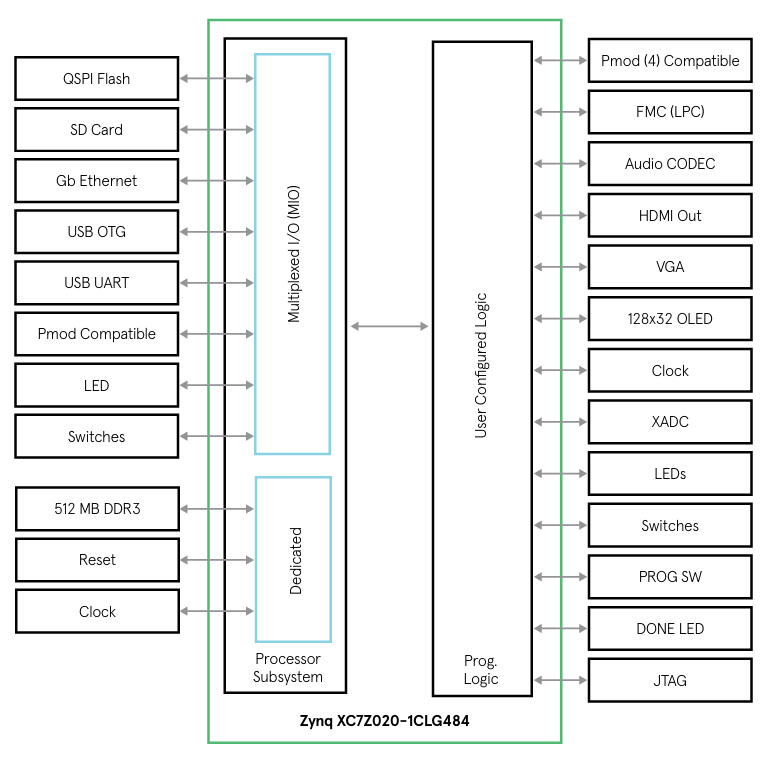
\includegraphics{images/zedboard_block_diagram.png}
\caption{Zedboard Block Diagram}
\end{figure}

\begin{quote}
An Inteltronic/Wisechip UG-2832HSWEG04 \textbf{OLED} Display is used on
the ZedBoard. This provides a 128x32 pixel, passive-matrix, monochrome
display. The display size is 30mm x 11.5mm x 1.45mm.
\end{quote}

\hypertarget{ug-2832hsweg04-oled-display}{%
\subsubsection{UG-2832HSWEG04 OLED
Display}\label{ug-2832hsweg04-oled-display}}

\hypertarget{oled-interface-pinout}{%
\paragraph{OLED Interface Pinout}\label{oled-interface-pinout}}

\begin{longtable}[]{@{}
  >{\raggedright\arraybackslash}p{(\columnwidth - 6\tabcolsep) * \real{0.1739}}
  >{\raggedright\arraybackslash}p{(\columnwidth - 6\tabcolsep) * \real{0.1159}}
  >{\raggedright\arraybackslash}p{(\columnwidth - 6\tabcolsep) * \real{0.1449}}
  >{\raggedright\arraybackslash}p{(\columnwidth - 6\tabcolsep) * \real{0.5652}}@{}}
\toprule\noalign{}
\begin{minipage}[b]{\linewidth}\raggedright
Pin Number
\end{minipage} & \begin{minipage}[b]{\linewidth}\raggedright
Symbol
\end{minipage} & \begin{minipage}[b]{\linewidth}\raggedright
Zynq Pin
\end{minipage} & \begin{minipage}[b]{\linewidth}\raggedright
Function
\end{minipage} \\
\midrule\noalign{}
\endhead
\bottomrule\noalign{}
\endlastfoot
\textbf{Interface} & & & \\
9 & RES\# & U9 & Power Reset for Controller and Driver \\
8 & CS\# & N/C & Chip Select -- Pulled Down on Board \\
10 & D/C\# & U10 & Data/Command Control \\
11 & SCLK & AB12 & Serial Clock Input Signal \\
12 & SDIN & AA12 & Serial Data Input Signal \\
\end{longtable}

The UG-2832HSWEG04 is a 0.91-inch OLED display module featuring a 128×32
pixel resolution and a 4-wire Serial Peripheral Interface (SPI) for
communication. This interface facilitates efficient data transfer
between the display module and a microcontroller.

\hypertarget{spi-interface-pins}{%
\paragraph{SPI Interface Pins}\label{spi-interface-pins}}

The display module utilizes the following pins for SPI communication:

\begin{itemize}
\tightlist
\item
  \textbf{CS\# (Chip Select):} Active-low input that enables the display
  module when pulled low.
\item
  \textbf{RES\# (Reset):} Active-low input that resets the display
  module when pulled low.
\item
  \textbf{D/C\# (Data/Command):} Determines the nature of the data; high
  for data, low for command.
\item
  \textbf{SCLK (Serial Clock):} Clock signal generated by the master
  device to synchronize data transmission.
\item
  \textbf{SDIN (Serial Data Input):} Serial data line for transmitting
  data from the master to the display module.
\end{itemize}

\hypertarget{communication-protocol}{%
\paragraph{Communication Protocol}\label{communication-protocol}}

\begin{enumerate}
\def\labelenumi{\arabic{enumi}.}
\tightlist
\item
  \textbf{Initialization:}

  \begin{itemize}
  \tightlist
  \item
    Pull \textbf{RES\#} low to reset the display module.
  \item
    Set \textbf{RES\#} high to complete the reset process.
  \end{itemize}
\item
  \textbf{Data Transmission:}

  \begin{itemize}
  \tightlist
  \item
    Set \textbf{CS\#} low to select the display module.
  \item
    Use \textbf{D/C\#} to specify the nature of the data:

    \begin{itemize}
    \tightlist
    \item
      Set \textbf{D/C\#} low for command bytes.
    \item
      Set \textbf{D/C\#} high for data bytes.
    \end{itemize}
  \item
    Transmit data via \textbf{SDIN}, synchronized with the \textbf{SCLK}
    signal. Data is latched on the rising edge of \textbf{SCLK}.
  \end{itemize}
\item
  \textbf{Termination:}

  \begin{itemize}
  \tightlist
  \item
    After data transmission, set \textbf{CS\#} high to deselect the
    display module.
  \end{itemize}
\end{enumerate}

\begin{figure}
\centering
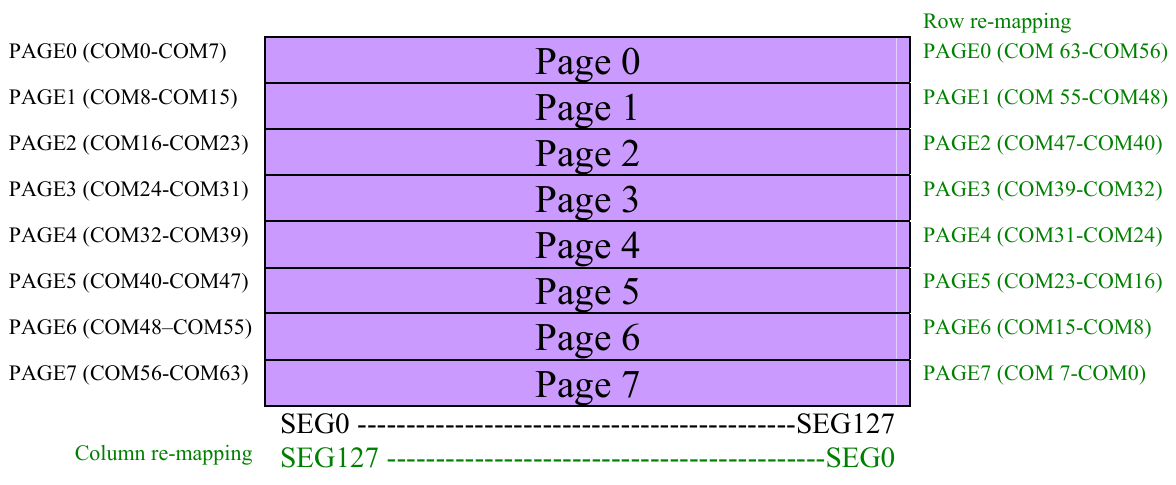
\includegraphics{images/gddram_page_structure.png}
\caption{GDDRAM Page Structure}
\end{figure}

\begin{figure}
\centering
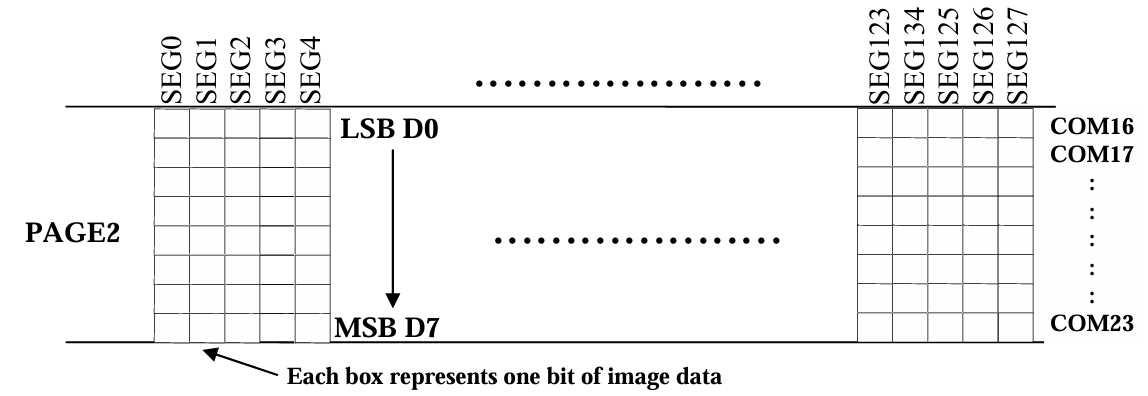
\includegraphics{images/gddram_page_breakdown.png}
\caption{GDDRAM Page Breakdown}
\end{figure}

\begin{center}\rule{0.5\linewidth}{0.5pt}\end{center}

References:

{[}1{]}
\href{https://www.avnet.com/wps/wcm/connect/onesite/557e3453-20d7-4737-b2a8-8afc404dc81e/designing_a_custom_axi_slave_rev1.pdf?MOD=AJPERES\&CVID=nxFlYvm\&CVID=nxFlYvm\&CVID=nxFlYvm\&CVID=nxFlYvm}{designing\_a\_custom\_axi\_slave\_rev1}

{[}2{]}
\href{https://www.avnet.com/wps/wcm/connect/onesite/922900e3-3d57-4cc7-883f-a8b9fbea0cd0/ZedBoard_HW_UG_v2_2.pdf?MOD=AJPERES\&CACHEID=ROOTWORKSPACE.Z18_NA5A1I41L0ICD0ABNDMDDG0000-922900e3-3d57-4cc7-883f-a8b9fbea0cd0-nxyWMFS}{ZedBoard\_HW\_Users\_Guide}

{[}3{]}
\href{https://cdn-shop.adafruit.com/datasheets/UG-2832HSWEG04.pdf}{OLED
Display Datasheet}

{[}4{]}
\href{https://cdn-shop.adafruit.com/datasheets/SSD1306.pdf}{SSD1306
Datasheet}
